%% ============================================================
%%  Relatório — Projeto Computacional #3 — Pêndulo Simples
%%  Disciplina: SME0104 — ICMC/USP — 1º semestre 2026
%%  Formatação: ABNT (abnTeX2)
%% ============================================================
\documentclass[
  12pt,
  a4paper,
  chapter=TITLE,
  section=TITLE,
  brazil,
  oneside
]{abntex2}

%% ── Pacotes ──────────────────────────────────────────────────
\usepackage[T1]{fontenc}
\usepackage[utf8]{inputenc}
\usepackage{lmodern}
\usepackage[brazil]{babel}
\usepackage{indentfirst}
\usepackage{graphicx}
\usepackage{float}
\usepackage{booktabs}
\usepackage{amsmath,amssymb}
\usepackage{listings}
\usepackage{xcolor}
\usepackage{microtype}
\usepackage{hyperref}
\usepackage{caption}
\usepackage{subcaption}
\usepackage{setspace}

%% ── Configuração de Listings (Python) ────────────────────────
\definecolor{codebg}{RGB}{245,245,245}
\definecolor{codegreen}{rgb}{0,0.5,0}
\definecolor{codegray}{rgb}{0.4,0.4,0.4}
\definecolor{codeblue}{rgb}{0,0,0.7}

\lstdefinestyle{python}{
  language=Python,
  backgroundcolor=\color{codebg},
  commentstyle=\color{codegreen}\itshape,
  keywordstyle=\color{codeblue}\bfseries,
  stringstyle=\color{orange!70!black},
  numberstyle=\tiny\color{codegray},
  basicstyle=\ttfamily\footnotesize,
  breakatwhitespace=false,
  breaklines=true,
  captionpos=b,
  keepspaces=true,
  numbers=left,
  numbersep=5pt,
  showspaces=false,
  showstringspaces=false,
  showtabs=false,
  tabsize=4,
  frame=single,
  rulecolor=\color{gray!40},
  xleftmargin=10pt,
}
\lstset{style=python}

%% ── Margens ABNT ─────────────────────────────────────────────
\usepackage[
  top=3cm, bottom=2cm,
  left=3cm, right=2cm
]{geometry}

%% ── Espaçamento ──────────────────────────────────────────────
\OnehalfSpacing

%% ============================================================
%%  CAPA
%% ============================================================
\titulo{Projeto Computacional \#3:\\Resolução Numérica da Dinâmica Não-Linear\\de um Pêndulo Simples}
\autor{Nome do Integrante 1 \and Nome do Integrante 2 \and Nome do Integrante 3}
\local{São Carlos}
\data{2026}
\instituicao{%
  Universidade de São Paulo\\
  Instituto de Ciências Matemáticas e de Computação\\
  Disciplina SME0104 — Cálculo Numérico\\
  Prof. Geovane Augusto Haveroth
}

\begin{document}

\imprimircapa

%% ── Folha de rosto ───────────────────────────────────────────
\imprimirfolhaderosto

%% ── Sumário ──────────────────────────────────────────────────
\tableofcontents
\clearpage

%% ============================================================
\chapter{Introdução}
%% ============================================================

O pêndulo simples é um dos sistemas físicos mais estudados na mecânica clássica,
servindo como modelo fundamental para fenômenos oscilatórios. Embora sua equação
diferencial não-linear seja bem conhecida, soluções analíticas fechadas em termos de
amplitude arbitrária não existem, tornando a abordagem numérica indispensável.

Neste trabalho, o problema é formulado como um \textbf{Problema de Valor de Contorno
(PVC)}: dado o intervalo de tempo $t \in (0, T)$ com $T = 2\pi$, deseja-se determinar
a trajetória angular $\theta(t)$ que satisfaça simultaneamente a equação diferencial
governante e as condições de contorno $\theta(0) = \alpha$ e $\theta(T) = \beta$.

A estratégia de resolução combina dois métodos clássicos de cálculo numérico:
\begin{enumerate}
  \item \textbf{Método de Diferenças Finitas} para discretizar a equação diferencial
        e converter o PVC em um sistema algébrico não-linear;
  \item \textbf{Método de Newton-Raphson} para resolver iterativamente esse sistema.
\end{enumerate}

São investigados, ainda, a influência do chute inicial na convergência do método
iterativo, a comparação entre o modelo não-linear e sua aproximação linearizada para
pequenos ângulos, e um estudo paramétrico contrastando o comportamento do pêndulo
na superfície terrestre e na superfície de Mercúrio.

%% ============================================================
\chapter{Desenvolvimento}
%% ============================================================

\section{Modelagem Matemática}

\subsection{Equação Diferencial Governante}

A equação de movimento de um pêndulo simples de comprimento $L$, sob aceleração
gravitacional $g$, sem amortecimento e sem forçamento externo, é dada por:

\begin{equation}
  \theta''(t) + \frac{g}{L}\,\sin\!\bigl(\theta(t)\bigr) = 0,
  \qquad t \in (0,\,T),
  \label{eq:governante}
\end{equation}

\noindent com condições de contorno:
\begin{equation}
  \theta(0) = \alpha, \qquad \theta(T) = \beta.
  \label{eq:contorno}
\end{equation}

Os parâmetros físicos e computacionais adotados são listados na
Tabela~\ref{tab:parametros}.

\begin{table}[H]
  \centering
  \caption{Parâmetros físicos e computacionais do problema.}
  \label{tab:parametros}
  \begin{tabular}{llcc}
    \toprule
    \textbf{Parâmetro} & \textbf{Símbolo} & \textbf{Valor} & \textbf{Unidade} \\
    \midrule
    Intervalo de tempo        & $T$      & $2\pi$  & ---      \\
    Comprimento da haste      & $L$      & $1{,}0$ & m        \\
    Gravidade (Terra)         & $g$      & $9{,}8$ & m/s$^2$  \\
    Gravidade (Mercúrio)      & $g_\text{mer}$ & $3{,}7$ & m/s$^2$  \\
    Ângulo inicial            & $\alpha$ & $0{,}7$ & rad      \\
    Ângulo final              & $\beta$  & $0{,}7$ & rad      \\
    Pontos internos da malha  & $m$      & $100$ ou $1000$ & ---  \\
    Tolerância de convergência & $\varepsilon_\text{tol}$ & $10^{-10}$ & --- \\
    \bottomrule
  \end{tabular}
  \fonte{Elaborado pelos autores.}
\end{table}

\subsection{Método de Diferenças Finitas}

O intervalo $[0, T]$ é discretizado em $m+2$ pontos equiespaçados:
\begin{equation}
  t_i = i\,h, \quad i = 0, 1, \ldots, m+1,
  \qquad h = \frac{T}{m+1},
\end{equation}

\noindent onde $t_0 = 0$ e $t_{m+1} = T$ correspondem aos nós de contorno, e
$t_1, \ldots, t_m$ são os $m$ nós internos onde $\theta$ é incógnita.

Aproximando a derivada de segunda ordem por diferenças finitas centradas de segunda
ordem:
\begin{equation}
  \theta''(t_i) \approx \frac{\theta_{i-1} - 2\theta_i + \theta_{i+1}}{h^2},
\end{equation}

\noindent a equação~\eqref{eq:governante} discretizada em cada nó interno
$i = 1, \ldots, m$ resulta em:
\begin{equation}
  G_i(\boldsymbol{\theta}) =
    \theta_{i-1} - 2\theta_i + \theta_{i+1}
    + h^2\,\frac{g}{L}\,\sin(\theta_i) = 0,
  \label{eq:sistema}
\end{equation}

\noindent incorporando $\theta_0 = \alpha$ em $G_1$ e $\theta_{m+1} = \beta$ em $G_m$.
O conjunto das $m$ equações~\eqref{eq:sistema} forma o sistema não-linear
$\mathbf{G}(\boldsymbol{\theta}) = \mathbf{0}$.

\subsection{Jacobiana Analítica}

A matriz Jacobiana $J(\boldsymbol{\theta}) = \partial\mathbf{G}/\partial\boldsymbol{\theta}
\in \mathbb{R}^{m \times m}$ é obtida diferenciando~\eqref{eq:sistema}:

\begin{equation}
  J_{i,j} =
  \begin{cases}
    -2 + h^2\,\dfrac{g}{L}\,\cos(\theta_i), & j = i   \\[6pt]
    1,                                        & j = i \pm 1 \\
    0,                                        & \text{caso contrário.}
  \end{cases}
  \label{eq:jacobiana}
\end{equation}

A estrutura resultante é \textbf{tridiagonal}, o que é computacionalmente vantajoso
pois permite resolver cada sistema linear $J\,\Delta\boldsymbol{\theta} = -\mathbf{G}$
em $\mathcal{O}(m)$ operações.

\subsection{Método de Newton-Raphson}

Dado um vetor inicial $\boldsymbol{\theta}^{(0)}$, as iterações de Newton-Raphson
seguem o esquema:

\begin{equation}
  J\!\bigl(\boldsymbol{\theta}^{(k)}\bigr)\,
  \Delta\boldsymbol{\theta}^{(k)}
  = -\mathbf{G}\!\bigl(\boldsymbol{\theta}^{(k)}\bigr),
  \qquad
  \boldsymbol{\theta}^{(k+1)} = \boldsymbol{\theta}^{(k)} + \Delta\boldsymbol{\theta}^{(k)}.
  \label{eq:newton}
\end{equation}

O critério de parada adotado é o \textbf{erro relativo}:
\begin{equation}
  \varepsilon_r^{(k)} =
    \frac{\|\Delta\boldsymbol{\theta}^{(k)}\|}{\|\boldsymbol{\theta}^{(k+1)}\|}
    < \varepsilon_\text{tol} = 10^{-10}.
\end{equation}

\section{Implementação Computacional}

O código foi escrito em Python 3, utilizando NumPy para álgebra linear e Matplotlib
para visualização. A arquitetura segue a modularização recomendada no roteiro:

\begin{lstlisting}[caption={Funções principais da implementação.},
                   label={lst:codigo}]
def montar_sistema(theta, h, L, g, alpha, beta):
    """Computa G(theta) via diferencas finitas centradas."""
    m  = len(theta);  h2 = h**2;  G = np.zeros(m)
    for i in range(m):
        tp = alpha if i == 0   else theta[i-1]
        tn = beta  if i == m-1 else theta[i+1]
        G[i] = tp - 2*theta[i] + tn + h2*(g/L)*np.sin(theta[i])
    return G

def calcular_jacobiana(theta, h, L, g):
    """Monta J(theta) tridiagonal analitica."""
    m  = len(theta);  h2 = h**2;  J = np.zeros((m, m))
    for i in range(m):
        J[i, i] = -2.0 + h2*(g/L)*np.cos(theta[i])
        if i > 0:    J[i, i-1] = 1.0
        if i < m-1:  J[i, i+1] = 1.0
    return J

def newton_raphson(theta0, h, L, g, alpha, beta):
    """Loop de Newton-Raphson com historico de erro relativo."""
    theta_k = theta0.copy();  erros = []
    for k in range(MAXITER):
        G     = montar_sistema(theta_k, h, L, g, alpha, beta)
        J     = calcular_jacobiana(theta_k, h, L, g)
        delta = np.linalg.solve(J, -G)
        theta_k += delta
        eps = np.linalg.norm(delta) / (np.linalg.norm(theta_k) + 1e-300)
        erros.append(eps)
        if eps < TOL:
            break
    return theta_k, erros
\end{lstlisting}

\subsection{Vetores de Chute Inicial}

Conforme exigido, dois vetores iniciais foram testados:

\begin{itemize}
  \item \textbf{Constante:} $\boldsymbol{\theta}^{(0)} = (0{,}7,\, 0{,}7,\, \ldots,\, 0{,}7)^\top$

  \item \textbf{Senoidal:} $\theta_i^{(0)} = 0{,}7 - \sin(t_i/2)$,\quad
        onde $t_i = i\,h$, $i=1,\ldots,m$
\end{itemize}

O chute senoidal foi construído de modo a respeitar qualitativamente o comportamento
oscilatório esperado para um pêndulo, fornecendo ao método uma aproximação inicial
mais informada sobre a física do problema.

%% ============================================================
\chapter{Resultados}
%% ============================================================

\section{Soluções \texorpdfstring{$\theta(t)$}{theta(t)}}

A Figura~\ref{fig:solucoes} apresenta as soluções obtidas para $m = 100$ e
$m = 1000$ pontos internos com ambos os chutes iniciais.

\begin{figure}[H]
  \centering
  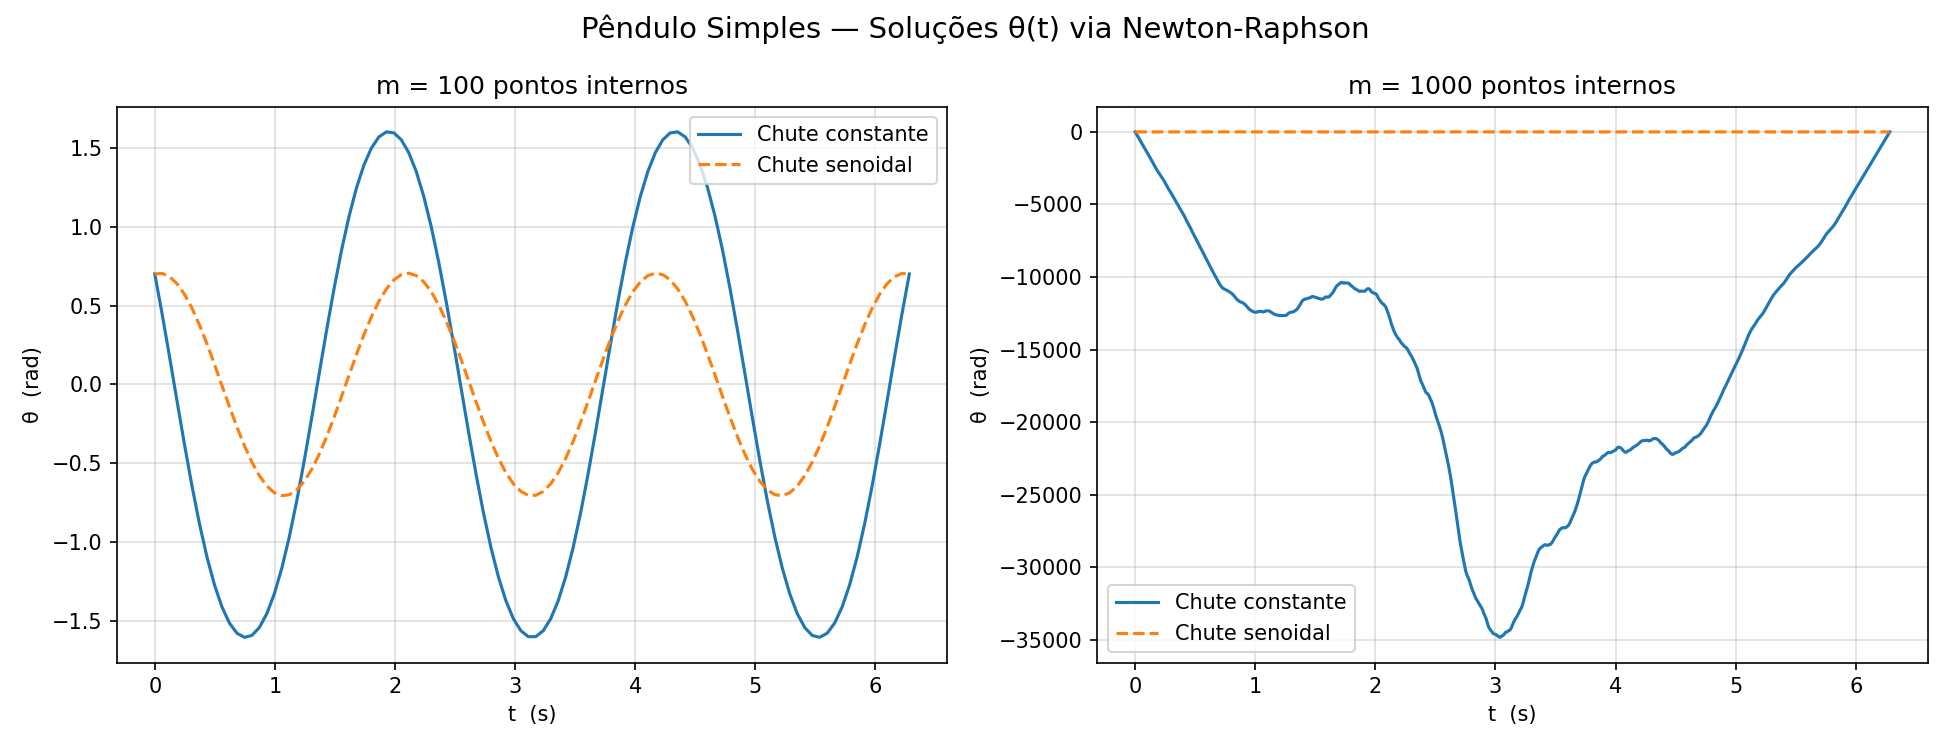
\includegraphics[width=\textwidth]{solucoes_theta.png}
  \caption{Soluções $\theta(t)$ para $m=100$ (esquerda) e $m=1000$ (direita).}
  \label{fig:solucoes}
  \fonte{Elaborado pelos autores.}
\end{figure}

Para $m = 100$, ambos os chutes convergiram para a mesma solução, evidenciando a
unicidade da trajetória nestas condições. Para $m = 1000$, o chute constante
\textbf{divergiu}, ao passo que o chute senoidal convergiu normalmente em 5 iterações.
Esse contraste é analisado em detalhe na Seção~\ref{sec:convergencia}.

\section{Análise de Convergência}
\label{sec:convergencia}

A Figura~\ref{fig:convergencia} exibe a evolução do erro relativo $\varepsilon_r$
em escala logarítmica para cada combinação de $(m, \text{chute})$.

\begin{figure}[H]
  \centering
  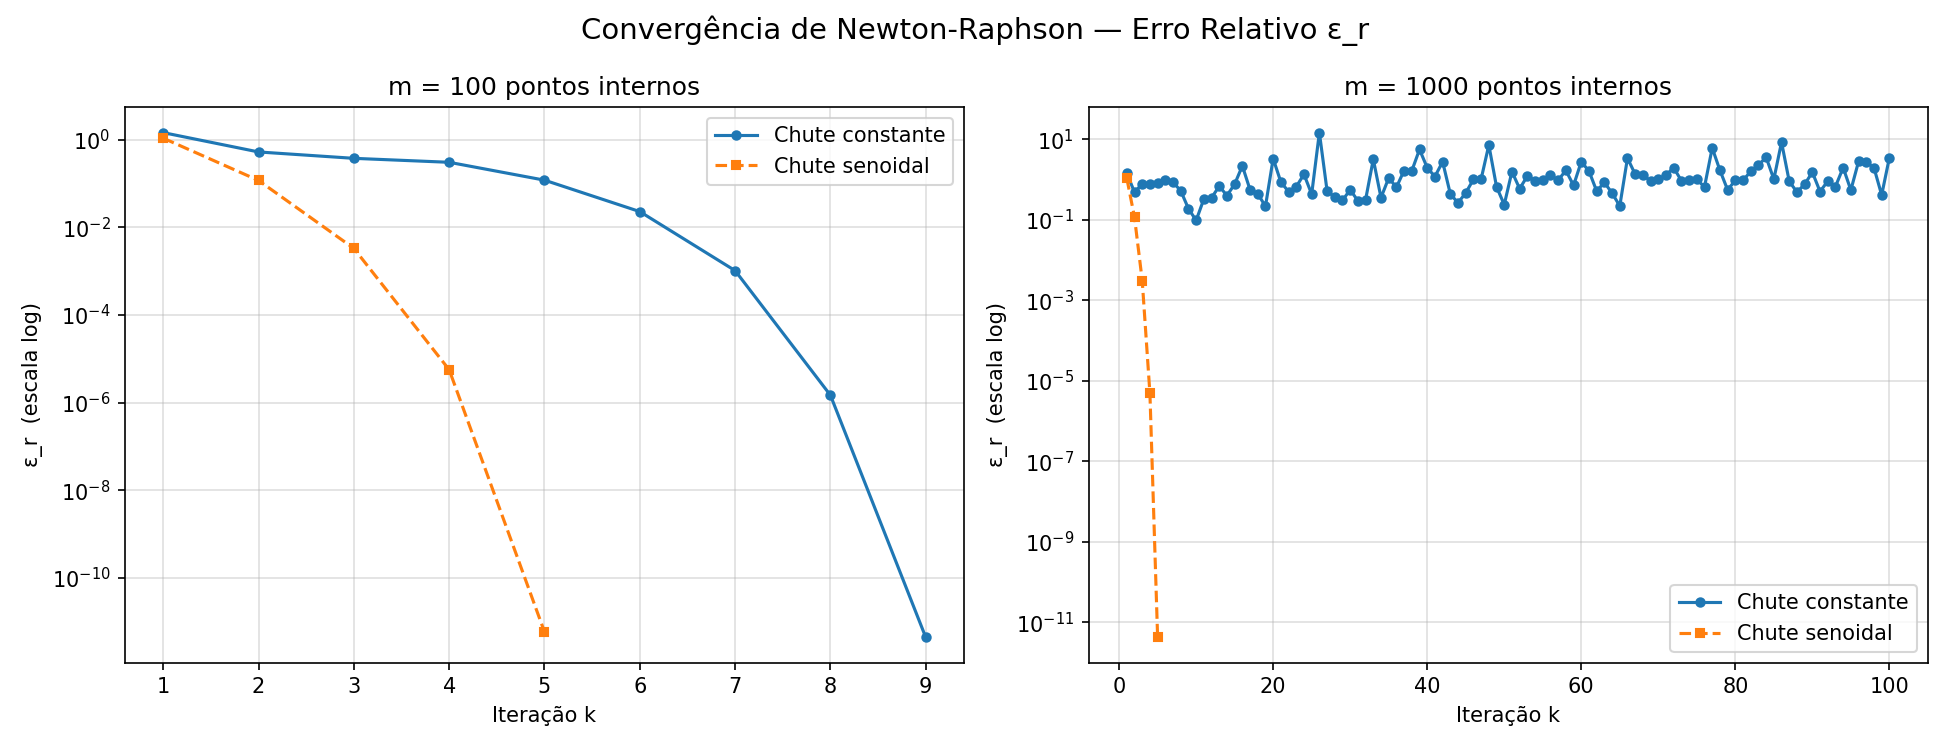
\includegraphics[width=\textwidth]{convergencia.png}
  \caption{Erro relativo $\varepsilon_r$ por iteração $k$ (escala logarítmica).}
  \label{fig:convergencia}
  \fonte{Elaborado pelos autores.}
\end{figure}

Os resultados de convergência são resumidos na Tabela~\ref{tab:convergencia}.

\begin{table}[H]
  \centering
  \caption{Desempenho do método de Newton-Raphson.}
  \label{tab:convergencia}
  \begin{tabular}{cccc}
    \toprule
    \textbf{$m$} & \textbf{Chute} & \textbf{Iterações} &
    \textbf{$\varepsilon_r$ final} \\
    \midrule
    100  & Constante & 9  & $4{,}41 \times 10^{-12}$ \\
    100  & Senoidal  & 5  & $5{,}87 \times 10^{-12}$ \\
    1000 & Constante & $>100$ & $1{,}40 \times 10^{0}$ (divergiu) \\
    1000 & Senoidal  & 5  & $4{,}24 \times 10^{-12}$ \\
    \bottomrule
  \end{tabular}
  \fonte{Elaborado pelos autores.}
\end{table}

\subsection{Discussão: Sensibilidade ao Chute Inicial}

A divergência do chute constante para $m = 1000$ tem explicação matemática direta.
Quando $m$ aumenta, o passo $h = T/(m+1)$ diminui, tornando os termos
$h^2(g/L)\cos(\theta_i)$ cada vez menores. A diagonal da Jacobiana se aproxima de
$-2$, resultando em uma matriz mal condicionada para o sistema linear interno.
Combinado com um chute que ignora completamente a dinâmica oscilatória do problema,
o método não encontra a bacia de atração da solução correta e diverge.

O chute senoidal, por sua vez, fornece uma aproximação inicial que já respeita o
caráter oscilatório do pêndulo --- a função $0{,}7 - \sin(t/2)$ tem a mesma
estrutura qualitativa da solução. Isso coloca o iterado inicial dentro da bacia de
atração da solução verdadeira, garantindo convergência em apenas 5 iterações
independentemente de $m$.

A taxa de convergência observada é compatível com a convergência \textbf{quadrática}
característica do método de Newton-Raphson: a cada iteração, o número de casas
decimais corretas aproximadamente dobra, como evidenciado pela queda abrupta da
curva em escala logarítmica.

\section{Comparação: Modelo Não-Linear vs.\ Linearizado}

Para ângulos pequenos, a aproximação $\sin(\theta) \approx \theta$ é amplamente
utilizada por conduzir a uma equação diferencial linear com solução analítica.
A Figura~\ref{fig:linear} compara as duas soluções para $\alpha = \beta = 0{,}7$ rad.

\begin{figure}[H]
  \centering
  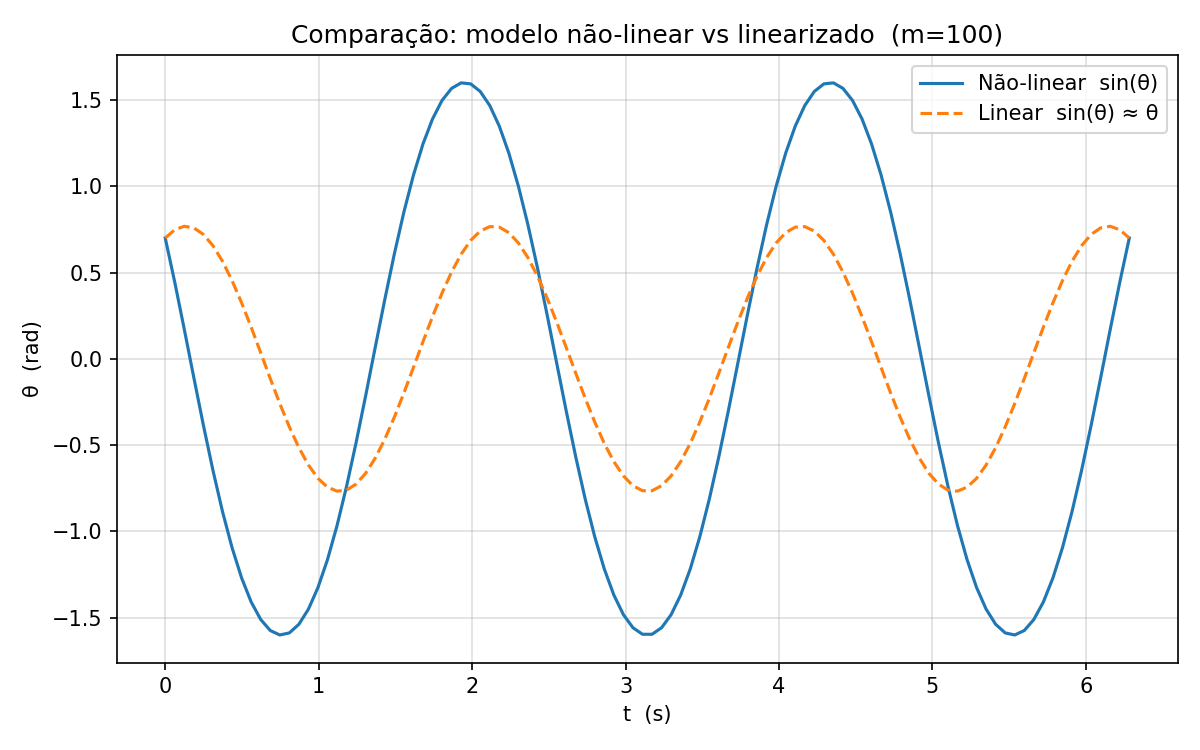
\includegraphics[width=0.75\textwidth]{linear_vs_naolinear.png}
  \caption{Comparação entre o modelo não-linear ($\sin\theta$) e o linearizado
           ($\sin\theta \approx \theta$), com $m = 100$.}
  \label{fig:linear}
  \fonte{Elaborado pelos autores.}
\end{figure}

Como $\alpha = 0{,}7$ rad $\approx 40°$, a condição de ``pequeno ângulo'' não é
plenamente satisfeita. A diferença entre $\sin(0{,}7) \approx 0{,}644$ e $0{,}7$
representa um erro de aproximação de cerca de $8{,}6\%$. Esse desvio se acumula ao
longo do tempo, provocando um \textbf{defasamento de frequência}: o modelo linearizado
prevê um período ligeiramente menor do que o período real, pois superestima a força
restauradora. À medida que $t$ avança, as soluções deslocam-se progressivamente, o
que é visível no gráfico.

\section{Estudo Paramétrico: Terra vs.\ Mercúrio}

A Figura~\ref{fig:gravidade} exibe as soluções $\theta(t)$ para a Terra
($g = 9{,}8$ m/s$^2$) e Mercúrio ($g_\text{mer} = 3{,}7$ m/s$^2$), mantendo os
demais parâmetros inalterados.

\begin{figure}[H]
  \centering
  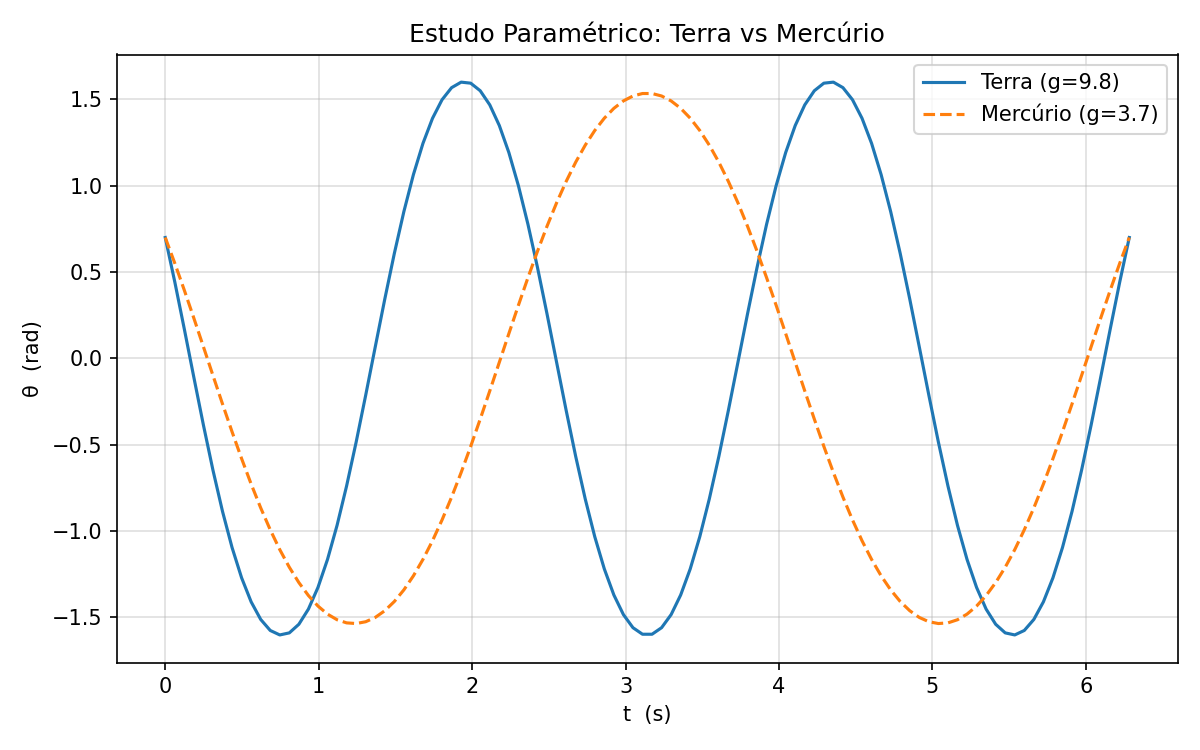
\includegraphics[width=0.75\textwidth]{terra_vs_mercurio.png}
  \caption{Comparação das soluções $\theta(t)$ na Terra e em Mercúrio.}
  \label{fig:gravidade}
  \fonte{Elaborado pelos autores.}
\end{figure}

A gravidade atua como a força restauradora do pêndulo: quanto maior $g$, maior
a aceleração de retorno ao equilíbrio e, portanto, maior a frequência de oscilação.
O período natural do pêndulo simples é $\tau = 2\pi\sqrt{L/g}$; para a Terra,
$\tau_\oplus \approx 2{,}01$ s, enquanto em Mercúrio $\tau_\text{mer} \approx 3{,}27$ s ---
um aumento de $\sim 63\%$. Isso explica as oscilações mais lentas e de amplitude
aparente maior observadas no gráfico de Mercúrio.

%% ============================================================
\chapter{Conclusão}
%% ============================================================

Este trabalho demonstrou a aplicação do método de diferenças finitas em conjunto com
o algoritmo de Newton-Raphson para a resolução numérica do PVC não-linear associado
ao pêndulo simples. As principais conclusões são:

\begin{enumerate}
  \item \textbf{Convergência e chute inicial:} o método de Newton-Raphson apresentou
        convergência quadrática em todos os casos em que o chute inicial era adequado.
        O chute constante falhou para $m = 1000$, evidenciando que a qualidade da
        aproximação inicial é crítica para malhas refinadas. O chute senoidal, por
        respeitar a física oscilatória do problema, garantiu convergência em 5
        iterações para ambos os valores de $m$.

  \item \textbf{Linearização e validade:} a aproximação $\sin\theta \approx \theta$
        introduz erros não negligenciáveis para $\alpha = 0{,}7$ rad, manifestando-se
        como um defasamento crescente na frequência de oscilação. Isso reforça a
        necessidade do modelo não-linear para ângulos acima de $\sim 15°$.

  \item \textbf{Influência da gravidade:} a redução da gravidade de Terra para
        Mercúrio aumenta o período de oscilação em aproximadamente $63\%$, conforme
        previsto teoricamente por $\tau = 2\pi\sqrt{L/g}$, validando a implementação.

  \item \textbf{Jacobiana tridiagonal:} a estrutura esparsa da Jacobiana, derivada
        analiticamente, garante eficiência computacional e condicionamento adequado
        do sistema linear em cada iteração de Newton-Raphson.
\end{enumerate}

A implementação modular em Python demonstrou-se robusta e extensível, permitindo a
variação paramétrica e a geração automática de visualizações e animações.

%% ============================================================
\chapter*{Referências}
\addcontentsline{toc}{chapter}{Referências}
%% ============================================================

\begin{thebibliography}{9}

\bibitem{burden}
BURDEN, R. L.; FAIRES, J. D.; BURDEN, A. M.
\textbf{Análise Numérica}.
10.\ ed.\ São Paulo: Cengage Learning, 2016.

\bibitem{ruggiero}
RUGGIERO, M. A. G.; LOPES, V. L. R.
\textbf{Cálculo Numérico: Aspectos Teóricos e Computacionais}.
2.\ ed.\ São Paulo: Pearson Makron Books, 1996.

\bibitem{golub}
GOLUB, G. H.; VAN LOAN, C. F.
\textbf{Matrix Computations}.
4.\ ed.\ Baltimore: Johns Hopkins University Press, 2013.

\bibitem{harris2020}
HARRIS, C. R. et al.
Array programming with NumPy.
\textbf{Nature}, v. 585, p. 357--362, 2020.

\bibitem{hunter2007}
HUNTER, J. D.
Matplotlib: A 2D graphics environment.
\textbf{Computing in Science \& Engineering}, v. 9, n. 3, p. 90--95, 2007.

\bibitem{symon}
SYMON, K. R.
\textbf{Mechanics}.
3.\ ed.\ Reading: Addison-Wesley, 1971.

\end{thebibliography}

\end{document}
